\section{Beweis der Funktionsfähigkeit}
In der Theorie funktionierte dieses Konstrukt bereits in Kapitel \ref{architektur}. Im Folgenden soll gezeigt werden, dass das entworfene Konstrukt aber auch in der Praxis relevante Werte liefert. Hierzu wird das in Kapitel \ref{numerschiesBeispiel} herangezogen, sowie ein standardisiertes Beispiel aus dem Themenbereich des \ac{TSP}, nämlich das a280-Problem - also eine Problemstellung mit 280 Städten.

\subsection{numerisches Beispiel}
In Abbildung \ref{tspAcoNumerisch} in Kapitel \ref{numerschiesBeispiel} wurde der Aufbau des numerischen Beispiels schon gezeigt. An der Ausgabe, welche beispielhaft in Abbildung \ref{numerischBeweis} als Ausschnitt der Log-Datei gezeigt ist, ist gut zu erkennen, dass schnell eine optimale Strecke gefunden werden konnte. 

Als Erinnerung: Bei der manuellen Berechnung des numerischen Beispiels belief sich die optimale Route auf eine Distanz von 29. Diese trat bei drei Ameisen nach drei Generationen auf. Zu Testzwecken lief das Programm nur mit einer Ameise, da bei einer zu hohen Anzahl an Ameisen bereits die erste Generation die optimale Strecke fand. Es lässt sich hiermit ableiten, dass die implementierte Architektur genauso abläuft wie das theoretische Konzept, wodurch eine fehlerfreie Implementierung bewiesen ist.

\begin{figure}[H]
	\centering
	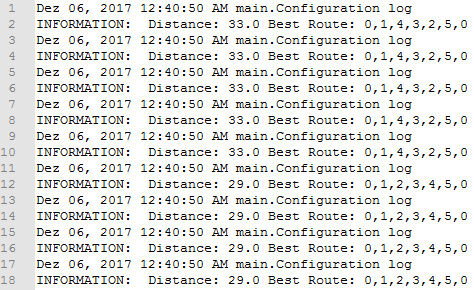
\includegraphics[width=0.6\linewidth]{images/numerischErgebnis.png}
	\caption{Ausschnitt der Log-Datei bei der Berechnung des numerischen Beispiels aus \ref{numerschiesBeispiel}. Jede Log-Zeile steht hier für eine Generation an Ameisen.}
	\label{numerischBeweis}
\end{figure}



\subsection{a280 drilling problem}
Aber nicht nur die fehlerfreie Implementierung soll bewiesen werden, sondern auch die Anwendungsmöglichkeiten auf komplexe Problemstellungen. Ohne diese Möglichkeit wäre das Programm darauf beschränkt die optimale Strecke innerhalb des numerischen Beispiels zu finden. Durch Abbildung \ref{drillingBeweis} lässt sich aber beweisen, dass auch deutlich größere Probleme sich berechnen lassen. Erkennbar sind mehrere Punkte:
\begin{itemize}
	\item Die Berechnungszeit wird etwas höher, erkennbar an dem Log-Zeitraum, der nun drei Sekunden umfasst
	\item Die Berechnungszeit beträgt immer noch deutlich weniger als eine Sekunde
	\item Es findet eine stetige Verbesserung der Distanz statt
\end{itemize}
Zusätzliche zu den Punkten lässt sich noch eine weitere Aussage ableiten: Das Problem lässt sich berechnen. Hierdurch ist der Punkt, der eigentlich bewiesen werden sollte, nachweislich belegt. Noch nicht bewiesen ist, ob der Algorithmus auch in kurzer Zeit ein Optimum finden kann. Da dieser Beweis allerdings mehr Hintergrundwissen und mehr Nachweise erfordert, wird dieser im späteren Kapitel \ref{proofOfConcept} behandelt.

\begin{figure}[H]
	\centering
	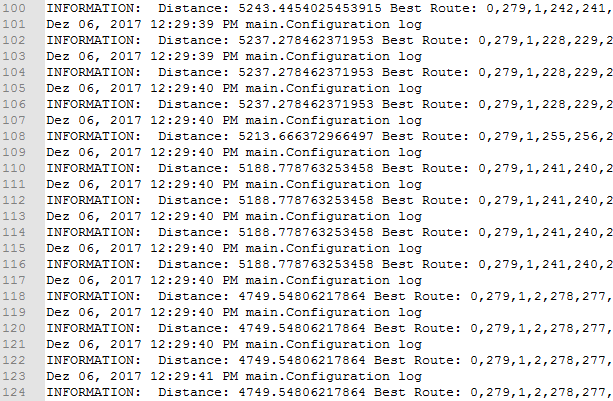
\includegraphics[width=0.6\linewidth]{images/a280Ergebnis.png}
	\caption{Ausschnitt der Log-Datei bei der Berechnung des ``a280 drilling problem''. Auch hier steht jede Log-Zeile für eine Generation an Ameisen.}
	\label{drillingBeweis}
\end{figure}